%
% File: chap03-03-01.tex
% Author: PINRU & LEONA
% Description:
% 3.3 Back-end Design and Implementations
%  3.3.1 API
%     Design
%     Implementation
%

\paragraph{Design}\mbox{}\\

In our virtual hospital website, the API works as a bridge between the frontend and the backend database. When we designed it, we mainly consider two things. One is the database rules, for example, username must be unique, and inputs should be checked. The second is the frontend use, like doctor or patient register and login, booking appointments, or searching hospital information. Since the request style is quite simple and mostly CRUD, we choose REST style and use Spring MVC.

For page rendering, we use Thymeleaf for server-side rendering. Something like GET /patient/manageAppointments will send back a HTML page with data already put inside. But when it is about actions that need fast response, like cancel appointment or refresh it, the frontend send AJAX to get JSON, for example POST /patient/appointments/cancel/{id} or GET /patient/appointments/refresh. Only part of the page will update, not reload the whole one. This mixed design, SSR for pages and JSON for small actions, makes first loading faster and user feeling smoother, and it is still not so complex.

To keep the API easy to use, we try to follow same rules for endpoint names, HTTP verbs and status code. Like GET is for reading data, POST for create, 200/201 for success, and clear error when validation fails. The controller will check important fields, like if password match or ID card and phone format. In the future, when database and permission are added, authentication and authorization can also be put under same endpoints, so frontend work flow will not be broken.

\paragraph{Implementation}\mbox{}\\

During the implementation, we used Spring Boot 3.5.3 with MyBatis for the database operation, which follows the patterns of a layered architecture \cite{fowler2002}. We are writing the actual API requests based on the API specification instructions.

The majority of the APIs are built similarly. For annotations like @GetMapping, we can set the kind of request type it is, the path it uses, and the response it gives back. The function then safely collects user details and passes them to the service layer methods, for them to handle the request.

Example code is shown below about the patient appointment information:

\begin{figure}[h]
\centering
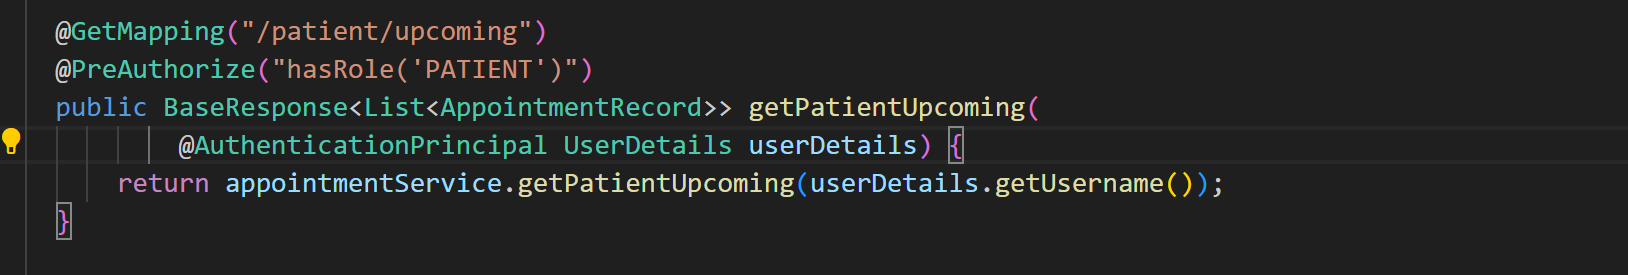
\includegraphics[width=0.8\textwidth]{chapters/chapter03/images03/3-3-1-figure(API-I).png}
\caption{Appointment Controller Implementation Code}
\label{fig:appointment-controller}
\end{figure}

Using @PreAuthorize, this will check the user's permissions and account levels \cite{springsecurity2024}. Using @AuthenticationPrincipal will then extract from Spring Security user information context; this doesn't need to authorise a token through a manual process \cite{johnson2023}.
The appointmentService.getPatientUpcoming() method includes dealing with business logic requests.

For the return type, we use \texttt{BaseResponse<T>}, replacing \texttt{ResponseEntity<ObjectNode>}, which offers the unified JSON structure. This type includes status code, message and data information, when dealing with different request errors, and the format makes it more consistent and clean.

Server methods contain business logic, and we use MyBatis to handle database operations \cite{springsecurity2024}. These functions create, update, delete, or query data through Mapper interfaces. MyBatis offer type-safe database operations and automatic SQL argument binding, compared to traditional JDBC, with fewer sample codes.

Some parts of server methods include more complicated logic, such as appointment scheduling, user personal information management, and health record handling. Those implementation methods not only enhance the optimisation, but also strengthen the system safety through Spring Security, integrate system safety, and provide a clear layer architecture to make the code more unified.
